\documentclass[11pt]{article}

\usepackage[a4paper, total={7in, 9.5in}]{geometry}
\usepackage{graphicx}
\usepackage{amssymb}
\usepackage{datetime}
\usepackage{pdfpages}
\usepackage{caption}
\usepackage{wrapfig}
\usepackage{tipa}
\usepackage{csvsimple}
\usepackage[T1]{fontenc}
\usepackage{hyperref}
\hypersetup{
	colorlinks=true,
	linkcolor=blue,
	filecolor=magenta,
	urlcolor=cyan,
	pdfpagemode=FullScreen,
}

\font\tenipa=tipa10
\def\schwa{{\tenipa\char64}}

\usepackage{array}
\newcolumntype{L}[1]{>{\raggedright\let\newline\\\arraybackslash\hspace{0pt}}p{#1}}
\newcolumntype{C}[1]{>{\centering\let\newline\\\arraybackslash\hspace{0pt}}p{#1}}
\newcolumntype{R}[1]{>{\raggedleft\let\newline\\\arraybackslash\hspace{0pt}}p{#1}}

\newdateformat{monthdayyeardate}{%
	\monthname[\THEMONTH]~\THEDAY, \THEYEAR}

\usepackage{setspace}
\usepackage{multirow}
\usepackage{xcolor}
\setlength{\parindent}{0em}
\setlength{\parskip}{0.5em}
\renewcommand{\baselinestretch}{1}

\begin{document}
\definecolor{myblue}{HTML}{3D4F7D}
\definecolor{myred}{HTML}{CD4F38}
\definecolor{mygreen}{HTML}{657060}
\definecolor{myorange}{HTML}{E48C2A}
\definecolor{mygreen2}{HTML}{44A57C}

\makebox[0pt][l]{%
  \raisebox{-\totalheight}[0pt][0pt]{%
  
\includegraphics{media/uvic.jpg}
  }}%


\hspace*{\fill}\textbf{Earth \& Ocean Sciences 408 CRN xxxxxx}\\
% (CRN 21332)
\hspace*{\fill}\textbf{UNIVERSITY OF VICTORIA}\\
\hspace*{\fill}\textbf{3-0-0 (1.5 UNITS)}\\
\hspace*{\fill}\textbf{FALL TERM 2025}\\


\noindent\hrulefill

\begin{center}
\emph{We acknowledge and respect the L\schwa\'k$^w$\schwa ŋ\schwa n (Songhees and Esquimalt) Peoples on whose territory the university stands, and the L\schwa\'k$^w$\schwa ŋ\schwa n and WS\'ANE\'C Peoples whose historical relationships with the land continue to this day.}
\end{center}

\noindent\hrulefill

\begin{center}
\Large \textbf{COURSE OUTLINE}

\Large \textbf{EOS408: Marine Geology}

\normalsize Lectures: M/Th 10:00 to 11:20 PM in MacLaurin D103 \\
\end{center}

\noindent\hrulefill

\textbf{PREREQUISITES}: EOS201, 1 of EOS310 or EOS316\\
\textbf{COREQUISITES}: NONE\\

\textbf{CONTACT INFO}

\begin{center}
  \centering
  \begin{tabular}{ L{.25\linewidth}L{.25\linewidth}L{.0\linewidth} }
    Instructor(s):      & Blake Dyer &  \\
    Email:      & blakedyer@uvic.ca &  \\
    Office:      & BWC A419 &  \\
    Office Hours:      & by appointment &  \\
          &  &  \\
    % Lab Coordinator      & none &  \\
Teaching Assistant(s):      & none &  \\
      &  &  \\
  \end{tabular}\\
\end{center}

\begin{center}
\textbf{COURSE DESCRIPTION}
\end{center}


In this course, we will explore geological processes in a wide range of oceanic environments: mid-ocean ridges, mid-plate volcanoes and hot spots, coastlines, continental margins and abyssal plains. The lectures, readings, and your writing will cover seminal scientific works and recent journal publications.
% KEY THEMES: [keywords]

\underline{This course is a science writing course.} Clear writing is one of the most important skills in science as it clarifies our own understanding of a topic and provides a pathway to communicate our ideas to others. \emph{You will be required to submit writing and revisions to your writing almost every week}. Your final grade in this course will largely reflect your ability to demonstrate your understanding of marine geology through your writing.

\clearpage

\textbf{LEARNING OUTCOMES}

Below is a list of some specific knowledge and skills you can expect to gain through this course. This term you will:
\begin{itemize}
	\setlength\itemsep{0em}
\csvreader[	head to column names, 
			before reading={\catcode`\"=9},
  			after reading={\catcode`\"=13}]
        {tables/learning_outcomes.csv}{1=\learningoutcome}
        {\item \learningoutcome}
\end{itemize}


\textbf{COURSE MATERIALS}

There is no required textbook. Readings will be made available through the course website.


\textbf{BRIGHTSPACE}

You are expected to routinely check the Brightspace site. All announcements, materials, readings, and schedule changes will be posted to brightspace.

\begin{center}
  \textbf{EVALUATION}
\end{center}

This course will use the \href{https://www.uvic.ca/calendar/future/undergrad/index.php#/policy/S1AAgoGuV?bc=true&bcCurrent=14%20-%20Grading&bcGroup=Undergraduate%20Academic%20Regulations&bcItemType=policies}{official UVic standard grading scale}. Your final grade will be determined by your scores on in-class preseentations, contributions to workshops, and writing submissions. There is no final exam.

\begin{center}
	\begin{tabular}{ L{.68\linewidth}R{.1\linewidth} R{.33\linewidth} }
		Participation and contributions to workshops & 12.5\% \\
		Review paper outline (Due Oct 13)            & 12.5\% \\
		Review paper first submission (Due Nov 17)   & 12.5\% \\
		Final paper submission (Due Dec 04)          & 42.5\% \\
		In class presentation                        & 22.5\% \\
	\end{tabular}
\end{center}

\textbf{EVALUATION: REVIEW PAPER}

Over the course of this term you will be writing a scientific review paper on a topic of your choosing within the scope of marine geology. The final paper should be between \textbf{2500 and 3500 words} and must have at least \textbf{two} original figures that you have created by combining data or concepts from your research. You will need to consult with the instructor and select an appropriate topic by Friday, September 22. We will be workshopping aspects of your paper and general science writing throughout the term. Your first submission of this review paper will be due on November 17. Your first submission will be reviewed by one of your peers for critical feedback. This feedback will be relayed back to you through the instructor and you will have the opportunity to respond and incorporate that feedback into your final submission on the last day of class, December 04. This review paper is a \textbf{required} component of the course. Failure to submit a review paper will result in a `N' grade.

\textbf{EVALUATION: PARTICIPATION AND CONTRIBUTION TO WORKSHOPS}

This course is at least half workshop-based, so it is especially important for everyone to participate and be heard.
You should be honest with your classmates and with the instructor, respectful toward everyone's thoughts and opinions, and compassionate toward your subject matter and the views of your peers.
A pattern of showing up to workshops unprepared will result in a zero for this aspect of your final grade.
More importantly, the workshops are designed to help you with the other graded aspects of the course, so failure to take advantage of the workshops will make it very tough to succeed in this course.
To get the most out of this course, you should:
\begin{itemize}
	\setlength\itemsep{0em}
	\item be on time and well-prepared for lectures and workshops.
	\item participate consistently and democratically in class, both by listening attentively
	      and contributing thoughtful comments and questions that build on classmates'
	      responses.
	\item speak not only to the professor but to other students; work energetically in small group or pair activities; overall, improve the day-to-day quality of the course for everyone.
	\item write cover letters that reflect thoughtfully and critically of your own writing.
	\item submit thoughtful and complete pre-workshop assignments and drafts.
	\item write peer review letters that offer fellow students substantive, constructive
	      feedback.
\end{itemize}

\textbf{EVALUATION: PRESENTATION} 

Towards the end of the term, you will give a 12 minute presentation for the class on the topic of your review paper. 

\begin{center}
  \textbf{COURSE POLICIES}
\end{center}

If you need academic accommodation to address barriers to your education, please register with the Centre for Accessible Learning (CAL) as soon as possible. We work with the CAL to create a learning environment that is equitable, inclusive, and usable for all.

\textbf{POLICY: CLASS CONDUCT}

Please follow the latest provincial and University guidelines with regard to COVID-19 protocols: \href{https://www.uvic.ca/covid19/index.php}{UVic COVID-19 information} and \href{https://www.uvic.ca/covid19/health-safety/index.php#ipn-if-you-re-sick}{what to do if you are ill}. No materials from the course may be redistributed without written permission from the instructors (e.g., no posting of materials to sharing websites). If we are required to meet on Zoom, you should remain muted during lecture unless you are speaking to the class or instructors.

\textbf{POLICY: LATE/MISSED ASSIGNMENTS OR EXAMINATIONS}

Assignment due dates are considered \textbf{hard deadlines}, except under extra-ordinary circumstances. If you have a known conflict that will make completing an assignment impossible, please notify the instructors well in advance of the due date.

\textbf{POLICY: ATTENDANCE}

You are expected to be present and active in the lectures and workshops. Missing workshops without communication and justification to the instructor will result in a lower final workshop score (refer to the rubric on Brightspace). Moreover, the workshops are designed to help you with your writing assignments, so missing workshops can indirectly hurt your writing scores. 

\textbf{POLICY: ACADEMIC INTEGRITY}

It is every student's responsibility to be aware of the university's \href{https://web.uvic.ca/calendar/undergrad/info/regulations/academic-integrity.html}{policies on ccademic integrity}, including policies on cheating, plagiarism, unauthorized use of an editor, multiple submission, and aiding others to cheat. 

If you have any questions or doubts, you can ask your course instructor or the \href{https://uvic.ca/learningandteaching/cac}{Centre for Academic Communication}.

\begin{center}
  \textbf{COURSE FEEDBACK}
\end{center}
\smallskip
\vspace*{-.6em}
I value your feedback on this course. Towards the end of term, as in all other courses at UVic, you will have the opportunity to complete an anonymous survey regarding your learning experience (CES). \textbf{The survey is vital for providing feedback} to me regarding the course and my teaching, as well as to help the department improve the overall program for students in the future. The survey is accessed online and can be done on your laptop, tablet, or mobile device. I will remind you and provide you with more detailed information nearer the time but please be thinking about this important activity during the course.

\begin{minipage}{\textwidth}
\begin{center}
  \textbf{COURSE WEEKLY CALENDAR}
\end{center}

This calendar will get updated throughout the term (last updated on: {\color{myred}\monthdayyeardate\today}). Exam dates are set, but lecture and lab topics are subject to change. 

\begin{tabular}{C{.06\linewidth}R{.12\linewidth}L{.76\linewidth}}
  \bfseries Week & \bfseries Date & \bfseries \hfill Lecture Topic\\
\csvreader[no head,late after line = \\]
        {tables/schedule.csv}{1=\wk,2=\dy,3=\mn,4=\daten,5=\subtcolor,6=\subt,7=\ltopic,8=\readings}
        {\bfseries \wk & \bfseries \dy~\mn~\daten & {\color{\subtcolor}\textbf{\subt}}\dotfill{\color{\subtcolor}\textbf{\ltopic}}}
\end{tabular}

\end{minipage}

\clearpage

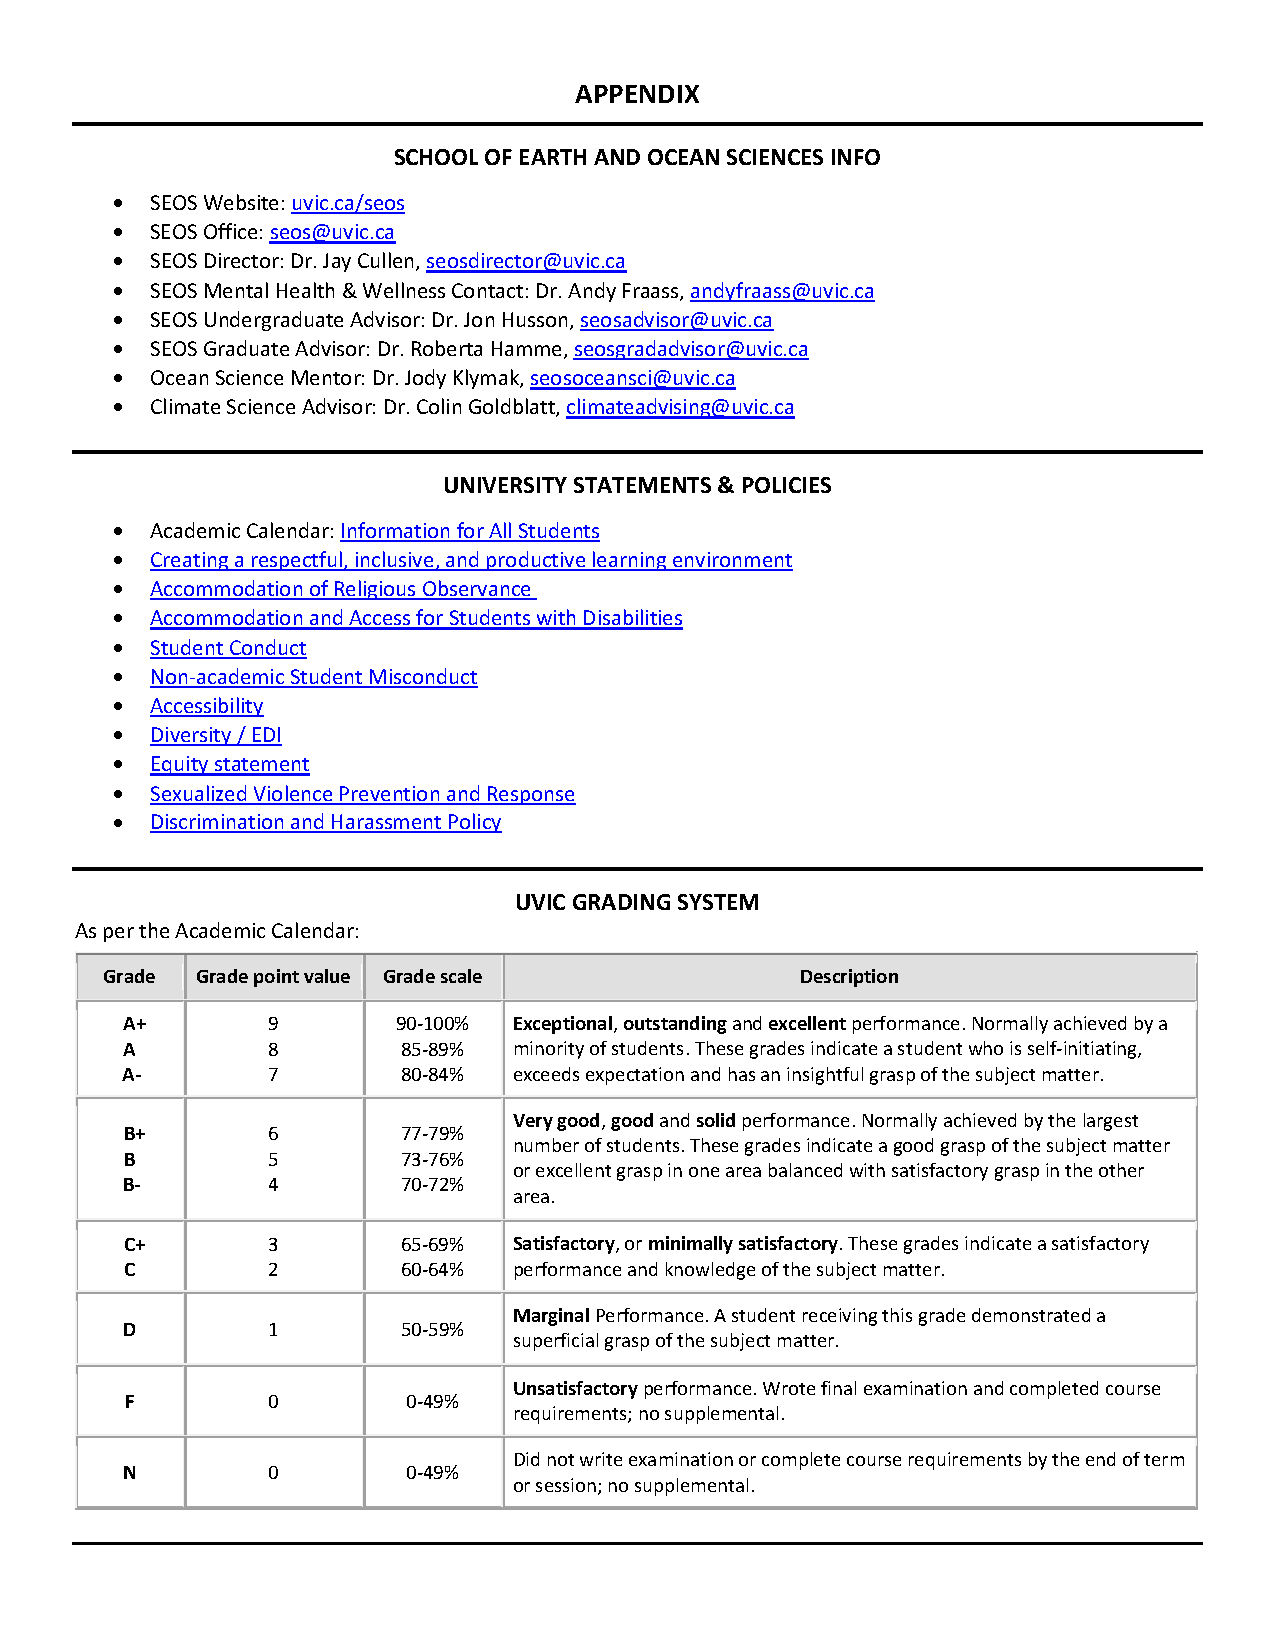
\includepdf[pages=-,pagecommand={},width=\textwidth]{Appendix.pdf}

\end{document}
